\documentclass[hyperref={pdfpagelabels=false}]{beamer}
% beamer already loads hyperref; do NOT load \usepackage{hyperref} again.

\usepackage{ragged2e} % 文字向兩邊對齊
\renewcommand{\raggedright}{\leftskip=0pt \rightskip=0pt plus 0cm}

\usepackage{listings}
\usepackage{lmodern}
\usepackage{fontspec}
\usepackage{xeCJK}
\setCJKmainfont{Noto Sans CJK TC}
%（可選）若你會用到無襯線中文或等寬中文，建議補上：
\setCJKsansfont{Noto Sans CJK TC}
\setCJKmonofont{Noto Sans Mono CJK TC}

\usepackage[english]{babel}
\usepackage{amsmath,amssymb,amsfonts,amsthm}

% hyperref settings (since beamer already loads hyperref)
\hypersetup{
  colorlinks=true,
  urlcolor=blue,
  citecolor=blue,
  pdfborder={0 0 0}
}

\usepackage{accsupp}% http://ctan.org/pkg/accsupp
\newcommand{\emptyaccsupp}[1]{\BeginAccSupp{ActualText={}}#1\EndAccSupp{}}

\usepackage{tikz}
\usetikzlibrary{arrows,decorations.pathmorphing,backgrounds,fit,positioning,shapes.symbols,chains}

\usepackage{booktabs}
\usepackage{threeparttable}
\usepackage{colortbl} 
\usepackage{xcolor}
\usetikzlibrary{tikzmark}

\newcommand{\indep}{\perp\!\!\!\perp}
\newcommand{\nindep}{\not\!\perp\!\!\!\perp}

\beamertemplatefootpagenumber


\usepackage{listings}
%%%%%%%%%%%%%%%%%%%%%%%%%%%%%%%%%%%%%%%%%%%%%%%%%%%%%%%%%%%%%%%%%%%%%%%%%%%%%%
% LaTeX snippet: language and style definition of Stata for listings package.
%                [listings](http://www.ctan.org/pkg/listings) 
%                [Stata](http://www.stata.com/)
%
% Usage:
%     Copy the code into your preamble, or import it by `\include` .
%     then in your doc:
%     \lstinputlisting[style=numbers]{DO-SCRIPT}
%     \lstinputlisting[style=numbers, style=stata-editor]{DO-SCRIPT}
%     \lstinputlisting[style=nonumbers, frame=none]{DO-SCRIPT}
% How it works:
%     - The language is defined by `\lstdefinelanguage{Stata}`
%     - Four styles is defined by `\lstdefinestyle{STYLE-NAME}`, 
%       they are: numbers and no numbers, plain(black and white) and colorful
%       (colored roughly like stata editor.)
% Tips:
%     - Generally you only need to set your default in the last part,
%       that is, code inside of `\lstset`.
%     - Add more keywords(I can not list all of them) in the `\lstset` part.
%     - Do NOT leave any blank lines in commands
%       (`\lstddefinelanguage', `\lstdefinestyle` and `\lstset`)
%
% update: 2014-04-16
% version: 0.1
% author: kongs
% licence: MIT
% url: https://gist.github.com/kongs-sublime/10862838
%
% TODO: 
%       - finish keyword list.
%       - precise colors that match stata editor?
%       - make it flexible(fonts and style)
%
%%%%%%%%%%%%%%%%%%%%%%%%%%%%%%%%%%%%%%%%%%%%%%%%%%%%%%%%%%%%%%%%%%%%%%%%%%%%%%


% langugae defination
\lstdefinelanguage{Stata}{
	% Left for users to add missing commands,
	% with possibility of choosing different style.
	morekeywords=,
	% Popular add-on commands
	morekeywords=[2]{cntrade, chinafin, 
		wbopendata, spmap,
	},
	% System commands
	morekeywords=[3]{regress, summarize, 
		display,
	},
	% Keywords
	morekeywords=[4]{forvalues, if, foreach, set},
	% Built-in functions
	morekeywords=[5]{rnormal, runiform},
	morecomment=[l]{//},
	% morecomment=[l]{*},  // `*` maybe used as multiply operator. So use `//` as line comment.
	morecomment=[s]{/*}{*/},
	% morecomment=[s]{,}{//},
	% The following is used by macros, like `lags'.
	morecomment=[n][keywordstyle9]{`}{'},
	morestring=[b]",
	sensitive=true,
}

\lstdefinestyle{numbers}{
	numbers=left, 
	stepnumber=1, 
	numberstyle=\tiny\emptyaccsupp,
	xleftmargin=2em,
}

\lstdefinestyle{nonumbers}{
	numbers=none,
}

\lstdefinestyle{stata-plain}{
	language=Stata,
	basicstyle=\footnotesize\ttfamily,
}

\lstdefinestyle{stata-editor}{
	language=Stata,
	basicstyle=\footnotesize\ttfamily,  
	keywordstyle={\color{NavyBlue}},  
	keywordstyle=[2]{\color{NavyBlue}},
	keywordstyle=[3]{\color{NavyBlue}},
	keywordstyle=[4]{\color{NavyBlue}},
	keywordstyle=[5]{\color{Blue}},
	keywordstyle=[9]{\color{TealBlue}},
	stringstyle=\color{Maroon},
	commentstyle=\color{OliveGreen},
}

\lstset{
	language=Stata,
	style=stata-plain,
	% style=stata-editor,
	style=numbers,
	showstringspaces=false,
	breaklines,
	frame=single,
	% To add missing commands
	% morekeywords={xtreg, xtunitroot},
}




\title[]  
{Shift-Share IV Design}

%\subtitle
%{免除部分負擔對幼兒醫療利用與健康的影響:斷點迴歸分析}

%\author 
%{Tzu-Ting Yang\inst{1} \and Hsing-Wen Han\inst{2} \and Hsien-Ming Lien\inst{3}}

%\institute[short]{\inst{1} Academia Sinica \and \inst{2} Tamkang University \and \inst{3} National Chengchi University}


\author 
{Prof. Tzu-Ting Yang  \\ 楊子霆}

%\institute{Institute of Economics, Academia Sinica  \\ Econ, NTU}
\institute{Institute of Economics, Academia Sinica  \\ 中央研究院經濟研究所}
%\institute{Institute of Economics, Academia Sinica  \\ Econ, NTU}
%\institute{Institute of Economics, Academia Sinica  \\ IMES/IDAS, NCCU}

%\author 
%{楊子霆 \\ 中研院經濟所}

%\institute 
%{中正大學國際經濟專題研討}




\date
{\today}


\usetheme{CambridgeUS}
%\usecolortheme{seahorse}
\setbeamertemplate{footline}{%
	\hfill\usebeamercolor[fg]{page number in head/foot}%
	\usebeamerfont{page number in head/foot}%
	\insertframenumber\,/\,\inserttotalframenumber\hspace{1em}\vspace{2pt}%
}

% \usetheme{Boadilla}
% %\useinnertheme{rectangles}

% %\usetheme{CambridgeUS}
% \usecolortheme{seahorse}
% \setbeamertemplate{footline}{%
% 	\hfill\usebeamercolor[fg]{page number in head/foot}%
% 	\usebeamerfont{page number in head/foot}%
% 	\insertframenumber\,/\,\inserttotalframenumber\hspace{1em}\vspace{2pt}%
% }


% \usepackage{beamerthemeshadow}
% %\usecolortheme{seahorse}
% \setbeamertemplate{footline}{%
% 	\hfill\usebeamercolor[fg]{page number in head/foot}%
% 	\usebeamerfont{page number in head/foot}%
% 	\insertframenumber\,/\,\inserttotalframenumber\hspace{1em}\vspace{2pt}%
% }


%\usepackage{beamerthemeshadow}

\beamersetuncovermixins{\opaqueness<1>{25}}{\opaqueness<2->{15}}

\begin{document}
	
	\begin{frame}
	\titlepage
\end{frame}


\title[]  
{Main Idea}


\author 
{}

%\institute{Institute of Economics, Academia Sinica  \\ Econ, NTU}
%\institute{Institute of Economics, Academia Sinica  \\ IMES/IDAS, NCCU}
\institute{}

%\author 
%{楊子霆 \\ 中研院經濟所}

%\institute 
%{中正大學國際經濟專題研討}




\date
{}


\begin{frame}{}
	\titlepage
\end{frame}





	\begin{frame}{Overview}
		\begin{itemize}
		\item The Shift-Share Instrumental Variable (SSIV) is a commonly used IV approach in econometrics to identify causal effects
								\vspace{0.2cm}
		\item It decomposes changes in economic variables within regions into two components: 
										\vspace{0.2cm}
	 \begin{itemize}
		\item \textbf{Shift}: Aggregate/external changes in economic variables across groups (e.g., industries, demographics)
																\vspace{0.2cm}		
		\item \textbf{Share}: Local area's initial exposure or composition of these groups
	\end{itemize}						
														\vspace{0.2cm}		
		\item First introduced by Bartik (1991), further developed and applied by Autor et al. (2013) and Kovak (2013)
								\vspace{0.2cm}
					\begin{itemize}					
		%\item Mainly used to study the impact of policies or shocks at the regional or industry level on micro-level individuals
		%								\vspace{0.2cm}
			\item Commonly applied in labor economics, trade, and economic geography
	\end{itemize}	
			
			
			
			
		\end{itemize}
	\end{frame}
	


	
%	\begin{frame}{Introduction}
%		\begin{itemize}
%			\item The Shift-Share Instrumental Variable (SSIV) combines shift-share analysis with instrumental variables to address endogeneity in economic models.
%			\item It leverages natural variations in industry composition across regions to identify causal effects of industry-specific shocks.
%		\end{itemize}
%	\end{frame}
	




	\begin{frame}{Motivating Example}{Impact of Robot on Labor Market Outcomes}
		\begin{itemize}
		\item We want to examine the effects of automation/robot on regional labor market by estimating the following regression
	\vspace{0.2cm}
	\begin{equation*}
		\Delta Y_{it} = \kappa + \beta \Delta R_{it} + X_{it-\tau} \gamma  + u_{it}
	\end{equation*}

		\item $\Delta Y_{it}$: Change in employment in the district $i$ over a long period 
		\vspace{0.2cm}
		\begin{itemize}	
			
			\item $\Delta$ represents long-run differences (e.g. 10 years, $\tau=10$)
			\vspace{0.2cm}
			\item 	$\Delta Y_{it} = Y_{it} - Y_{it-\tau}$
			\vspace{0.2cm}
			\item $Y_{it}$ represents total employment or average wage					
		\end{itemize}	
	
		%	\vspace{0.2cm}
		%		\item Includes district $\xi_{i}$ and time $\tau_{t}$ fixed effects to account for regional and temporal variations
		%		
		%		+ \xi_{i} + \tau_{t}
	\end{itemize}
\end{frame}






	\begin{frame}{Motivating Example}{Impact of Robot on Labor Market Outcomes}


	\begin{equation*}
		\Delta Y_{it} = \kappa + \beta \Delta R_{it} + X_{it-\tau} \gamma  + u_{it}
	\end{equation*}
	\begin{itemize}
		
		\item $\Delta R_{it}$: Change in robot exposure measure in the district $i$ over a long period
			\begin{itemize}
									\vspace{0.2cm}	
	\item 	$\Delta R_{it} = R_{it} - R_{it-\tau}$												\vspace{0.2cm}

\item $R_{it}$ represents robot stock
	%\vspace{0.2cm}
		%\item $\beta$: Impact of robot exposure on employment
			\end{itemize}
		
														\vspace{0.2cm}
		\item $X_{it-\tau}$: Control variables at district level in the baseline period $t-\tau$
															%	\vspace{0.2cm}
%		\item Includes district $\xi_{i}$ and time $\tau_{t}$ fixed effects to account for regional and temporal variations
%		
%		+ \xi_{i} + \tau_{t}
	\end{itemize}
\end{frame}



	\begin{frame}{Motivating Example}{Impact of Robot on Labor Market Outcomes}
	
	
	\begin{equation*}
		\Delta Y_{it} = \kappa + \beta \Delta R_{it} + X_{it-\tau} \gamma  + u_{it}
	\end{equation*}
	\begin{itemize}
		
		\item $\beta$: Impact of robot exposure on labor market outcomes
					\vspace{0.2cm}
		
			\item \textbf{Challenge:} Isolating the effect of robot exposure from other regional economic factors										
		\begin{itemize}
			
			\vspace{0.2cm}
			\item  Observed robot stock is endogenous to labor market conditions
			\vspace{0.2cm}
			\item  The increases in product demand for the factories in Hsinchu city would increase both the employment/wage and robot stock of the area
			
		\end{itemize}
		
		
	\end{itemize}
\end{frame}








\begin{frame}{Deriving the Shift-Share IV} 
	\begin{itemize}
		\item We can decompose the endogenous variable, $\Delta R_{it}$, as a weighted average of industry-specific changes:
		
		\begin{align*}
			\Delta R_{it} &\approx\sum_{k=1}^{N} \overbrace{\Delta R_{ikt}}^{\text{shift}} \times \overbrace{\frac{L_{ikt}}{L_{it}}}^{\text{share}} \\
			&\approx \Delta R_{i1t} \times \frac{L_{i1t}}{L_{it}} + \Delta R_{i2t} \times \frac{L_{i2t}}{L_{it}} + \cdots + \Delta R_{iNt} \times \frac{L_{iNt}}{L_{it}}
		\end{align*}
		%\vspace{0.2cm}
		
		\begin{itemize}
			\item $k = 1,2,\ldots,N$ indexes the industries in the economy
			\vspace{0.2cm}
			\item $\frac{L_{ikt}}{L_{it}}$ is industry $k$'s employment share in region $i$ at time $t$ 
			\vspace{0.2cm}
			\item $\Delta R_{ikt}$ is the change in outcome for industry $k$ in region $i$ 
			\vspace{0.2cm}
		%	\item $\Delta R_{it}$ likely confounds with unobserved factors, necessitating an IV
		%	\vspace{0.2cm}
			\item This is an approximation, not an identity. It holds closely only if employment shares are relatively stable between $t-\tau$ and $t$
		\end{itemize}
	\end{itemize}
\end{frame}


\begin{frame}{Derive Shift-Share IV}{Step 1}
	\textbf{Step 1:} Delocalization Shift IV
							\vspace{0.2cm}
	\begin{itemize}
		\item Replace the original \textbf{shift part}, $\Delta R_{ikt}$, by the \textbf{global/national change} $\Delta R_{kt}$ 
			\begin{itemize}
									\vspace{0.2cm}
		\item The national change in robot stock for a industry $k$
			\end{itemize}

	\[ \Delta Z_{it}=\sum_{k=1}^{N} \overbrace{\Delta R_{kt}}^{shift} \times  \overbrace{\frac{L_{ikt}}{L_{it}}}^{share} \]


\item Sometimes $\Delta R_{kt}$ may be $\Delta R_{kt,-i}$. It's the global change calculated without district i's values.
	\end{itemize}

\end{frame}



\begin{frame}{Derive Shift-Share IV}{Step 2}
	
	\textbf{Step 2:} Shift-Share IV
								\vspace{0.2cm}
	\begin{itemize}
		\item We add one more revision to the time period t of the \textbf{share part}: 
										\vspace{0.2cm}
			\begin{itemize}
		\item Replace it by some rules. E.g., frozen Lag (use base period's share), updating lag, averaging all periods. 
			\end{itemize}
	\end{itemize}
	\[ \Delta Z_{it}=\sum_{k} \overbrace{\Delta R_{kt}}^{shift} \times \overbrace{\frac{L_{ikt-\tau}}{L_{it-\tau}}}^{share} \]
\end{frame}


%\subsection{Derive SSIV-3}
%
%\begin{frame}{Derive SSIV-3}
%	\begin{itemize}
%		\item Note 1: Sometimes $\Delta R_{ikt}$ may be $\Delta R_{kt,-i}$. It's the global average calculated without district i’s values.
%		\item Note 2: At first glance, the source of variation in SSIV comes from the share part since the shift part is common for all districts in time t. (recent development has other interpretations)
%	\end{itemize}
%\end{frame}



\begin{frame}{Why Shift-Share IV Wokrs?}{Intuition}
	\begin{itemize}
		\item \textbf{De-localizing shift} should be able to remove the main part that causes selection bias
														\vspace{0.2cm}
			\begin{itemize}
		\item Use the national/global changes that cannot be affected (at least not too much) by the local factors to replace the shift.
										\end{itemize}			
		
		
												\vspace{0.2cm}
		\item But, the \textbf{share part} may be affected by confounders.
												\vspace{0.2cm}
													\begin{itemize}
		\item Therefore, we may use \textbf{Frozen Lag} (a base period's share), an \textbf{Updating Share} (use t-k share), or \textbf{averaging share}
										\vspace{0.2cm}
		\item Make sure the IV is \textbf{totally prior to the current period}
										\vspace{0.2cm}
								\end{itemize}			
		\item Intuitively, we want the \textbf{share part} to reflect that district's geographical or historical features that cannot be easily affected
	\end{itemize}
%	\small
%	Ferri (2022) P36: "For example, shipping relies on access to water, and locations are bound to particular industries, such as Detroit to manufacturing, for historical reasons that cannot be easily adjusted.”
\end{frame}

\begin{frame}{Why Shift-Share IV Wokrs?}{3 Ways to Adjust the Share}
	\begin{itemize}

	\item \textbf{Method 1: Frozen Lag}
			\vspace{0.2cm}
	\begin{itemize}
		\item Construct share using the value in first period $t=0$
							\vspace{0.2cm}
		\item So the first period of the panel is dropped
				\vspace{0.2cm}
				\end{itemize}		
		\item Downside:
				\vspace{0.2cm}
		\begin{itemize}
			\item Because the first period t=0 has a different distance from each t in the panel, the later periods are likely to be less relevant to $t=0$ time period.
		\end{itemize}
		
	\end{itemize}
	

\end{frame}




\begin{frame}{Why Shift-Share IV Wokrs?}{3 Ways to Adjust the Share}
	\begin{itemize}
	
	\item \textbf{Method 2: Updating Lag}
			\vspace{0.2cm}
	\begin{itemize}
		%\item Updating Lags rather maintain a common distance $\tau$ in time between each t and its lag
			%	\vspace{0.2cm}
		\item Construct share using the value in period $t-\tau$
		\vspace{0.2cm}
		\item Update share every $\tau$ periods
				\vspace{0.2cm}
		\item $\tau$ is a fixed number
	\end{itemize}

	\end{itemize}
\end{frame}


\begin{frame}{Why Shift-Share IV Wokrs?}{3 Ways to Adjust the Share}
		\begin{itemize}
	\item \textbf{Method 3: Averaging over all periods}
			\vspace{0.2cm}
	\begin{itemize}
		\item Construct share using the average value during all periods
			\vspace{0.2cm}

			\item With a large number of time periods, that is, the role of any one time period's values is minor

		
		\end{itemize}

	\end{itemize}
\end{frame}






\begin{frame}{Why Shift-Share IV Works?}
	\[ \Delta Z_{it}=\sum_{k=1}^{N} \overbrace{\Delta R_{kt}}^{\text{shift}} \times \overbrace{\frac{L_{ik,t-\tau}}{L_{i,t-\tau}}}^{\text{share}} \]
	\begin{itemize}
		\item \textbf{First-stage Relevance}: National/global changes ($\Delta R_{kt}$) are strongly correlated with local changes ($\Delta R_{ikt}$)
		\vspace{0.2cm}
		\item \textbf{Exclusion Restriction}: For validity, the instrument should affect outcomes only through the endogenous variable
				\vspace{0.2cm}
		\begin{itemize}
			\item Historical shares ($\frac{L_{ik,t-\tau}}{L_{i,t-\tau}}$) are predetermined, reducing concerns about simultaneity
					\vspace{0.2cm}
			\item National shifts ($\Delta R_{kt}$) are assumed to be exogenous to local conditions
		\end{itemize}
	\end{itemize}
\end{frame}

\begin{frame}{Potential Threats to SSIV Validity}
	\begin{itemize}
		\item The exclusion restriction may fail for several reasons:
		\vspace{0.2cm}
		\begin{itemize}
			\item \textbf{Persistent local shocks}: Historical industry shares may correlate with unobserved local characteristics that affect both past and current outcomes
			\vspace{0.2cm}
			\item \textbf{Feedback effects}: Large regions might influence national shifts, violating the exogeneity assumption (especially relevant for large metropolitan areas)
			\vspace{0.2cm}
			%\item \textbf{Multiple causal pathways}: National shifts may affect local outcomes through channels beyond the endogenous variable of interest
			%\vspace{0.2cm}
			%\item \textbf{Correlated industry shocks}: If industries experiencing similar shocks tend to cluster geographically
		\end{itemize}
		\vspace{0.3cm}
		\item Despite these challenges, SSIV remains valuable for addressing \textbf{reverse causality} and some forms of \textbf{omitted variable bias}
	%	\vspace{0.2cm}
		%\item Modern approaches: Leave-one-out estimators, controls for initial conditions, and industry-level standard errors
	\end{itemize}
\end{frame}




	
	\begin{frame}{Estimation Approach}{Two-stage Least-squares Regression }
		\begin{itemize}
			\item \textbf{First Stage Regression:}
			\begin{equation*}
			\Delta R_{it} = \lambda + \alpha \Delta Z_{it} + X_{it-\tau} \theta +  \epsilon_{it}
		\end{equation*}
			\item \textbf{Second Stage Regression:}
			\begin{equation*}
			\Delta Y_{it} =  \kappa + \beta \Delta \hat{R}_{it} + X_{it-\tau} \gamma + u_{it}
		\end{equation*}
	
	\item Use shift-share as IV for treatment variable $\Delta R_{it}$
	
	\[ \Delta Z_{it}=\sum_{k=1}^{N} \overbrace{\Delta R_{kt}}^{shift} \times \overbrace{\frac{L_{ikt-\tau}}{L_{it-\tau}}}^{share} \]
		%	\item Here, \(\hat{T}\) is the predicted level of automation from the first stage.
		\end{itemize}
	\end{frame}





\begin{frame}{Relevant Jargons}
	\begin{itemize}
		\item \textbf{A summary of relevant jargons}
		\vspace{0.2cm}
		\begin{itemize}
			\item Exposure Design $\approx$ SSIV = Bartik IV 
					\vspace{0.2cm}
					\begin{itemize}
			\item Because Bartik proposed this IV
			
					\end{itemize}
			\vspace{0.2cm}
			\item Shock = Shift
			\vspace{0.2cm}
			\item Some may say: "use predicted value to instrument the endogenous var..." since the SSIV is like a predicted value of the endogenous var.
		\end{itemize}
	\end{itemize}
\end{frame}





\title[]  
{Empirical Example}


\author 
{}

%\institute{Institute of Economics, Academia Sinica  \\ Econ, NTU}
%\institute{Institute of Economics, Academia Sinica  \\ IMES/IDAS, NCCU}
\institute{}

%\author 
%{楊子霆 \\ 中研院經濟所}

%\institute 
%{中正大學國際經濟專題研討}




\date
{}


\begin{frame}{}
	\titlepage
\end{frame}



\begin{frame}{Autor, David Dorn, and Gordon H. Hanson (2013)}
Autor, David H., David Dorn, and Gordon H. Hanson. "\textbf{The China syndrome: Local labor market effects of import competition in the United States.}" \textit{American Economic Review} 103.6 (2013): 2121-2168.
	\begin{itemize}
		\vspace{0.2cm}
		
			\item The paper examines the impact of increased Chinese import competition between 1990 and 2007 on local U.S. labor markets.
					\vspace{0.2cm}
		\item Utilizes a shift-share IV strategy to identify the effects of import competition.
				\vspace{0.2cm}
		\item Key findings suggest significant impacts on employment, wages, and the receipt of welfare benefits in regions more exposed to import competition.
	\end{itemize}
\end{frame}



\begin{frame}{Graphical Evidence}{}
	
	\begin{center}
		\begin{figure}[p]
			\centering
			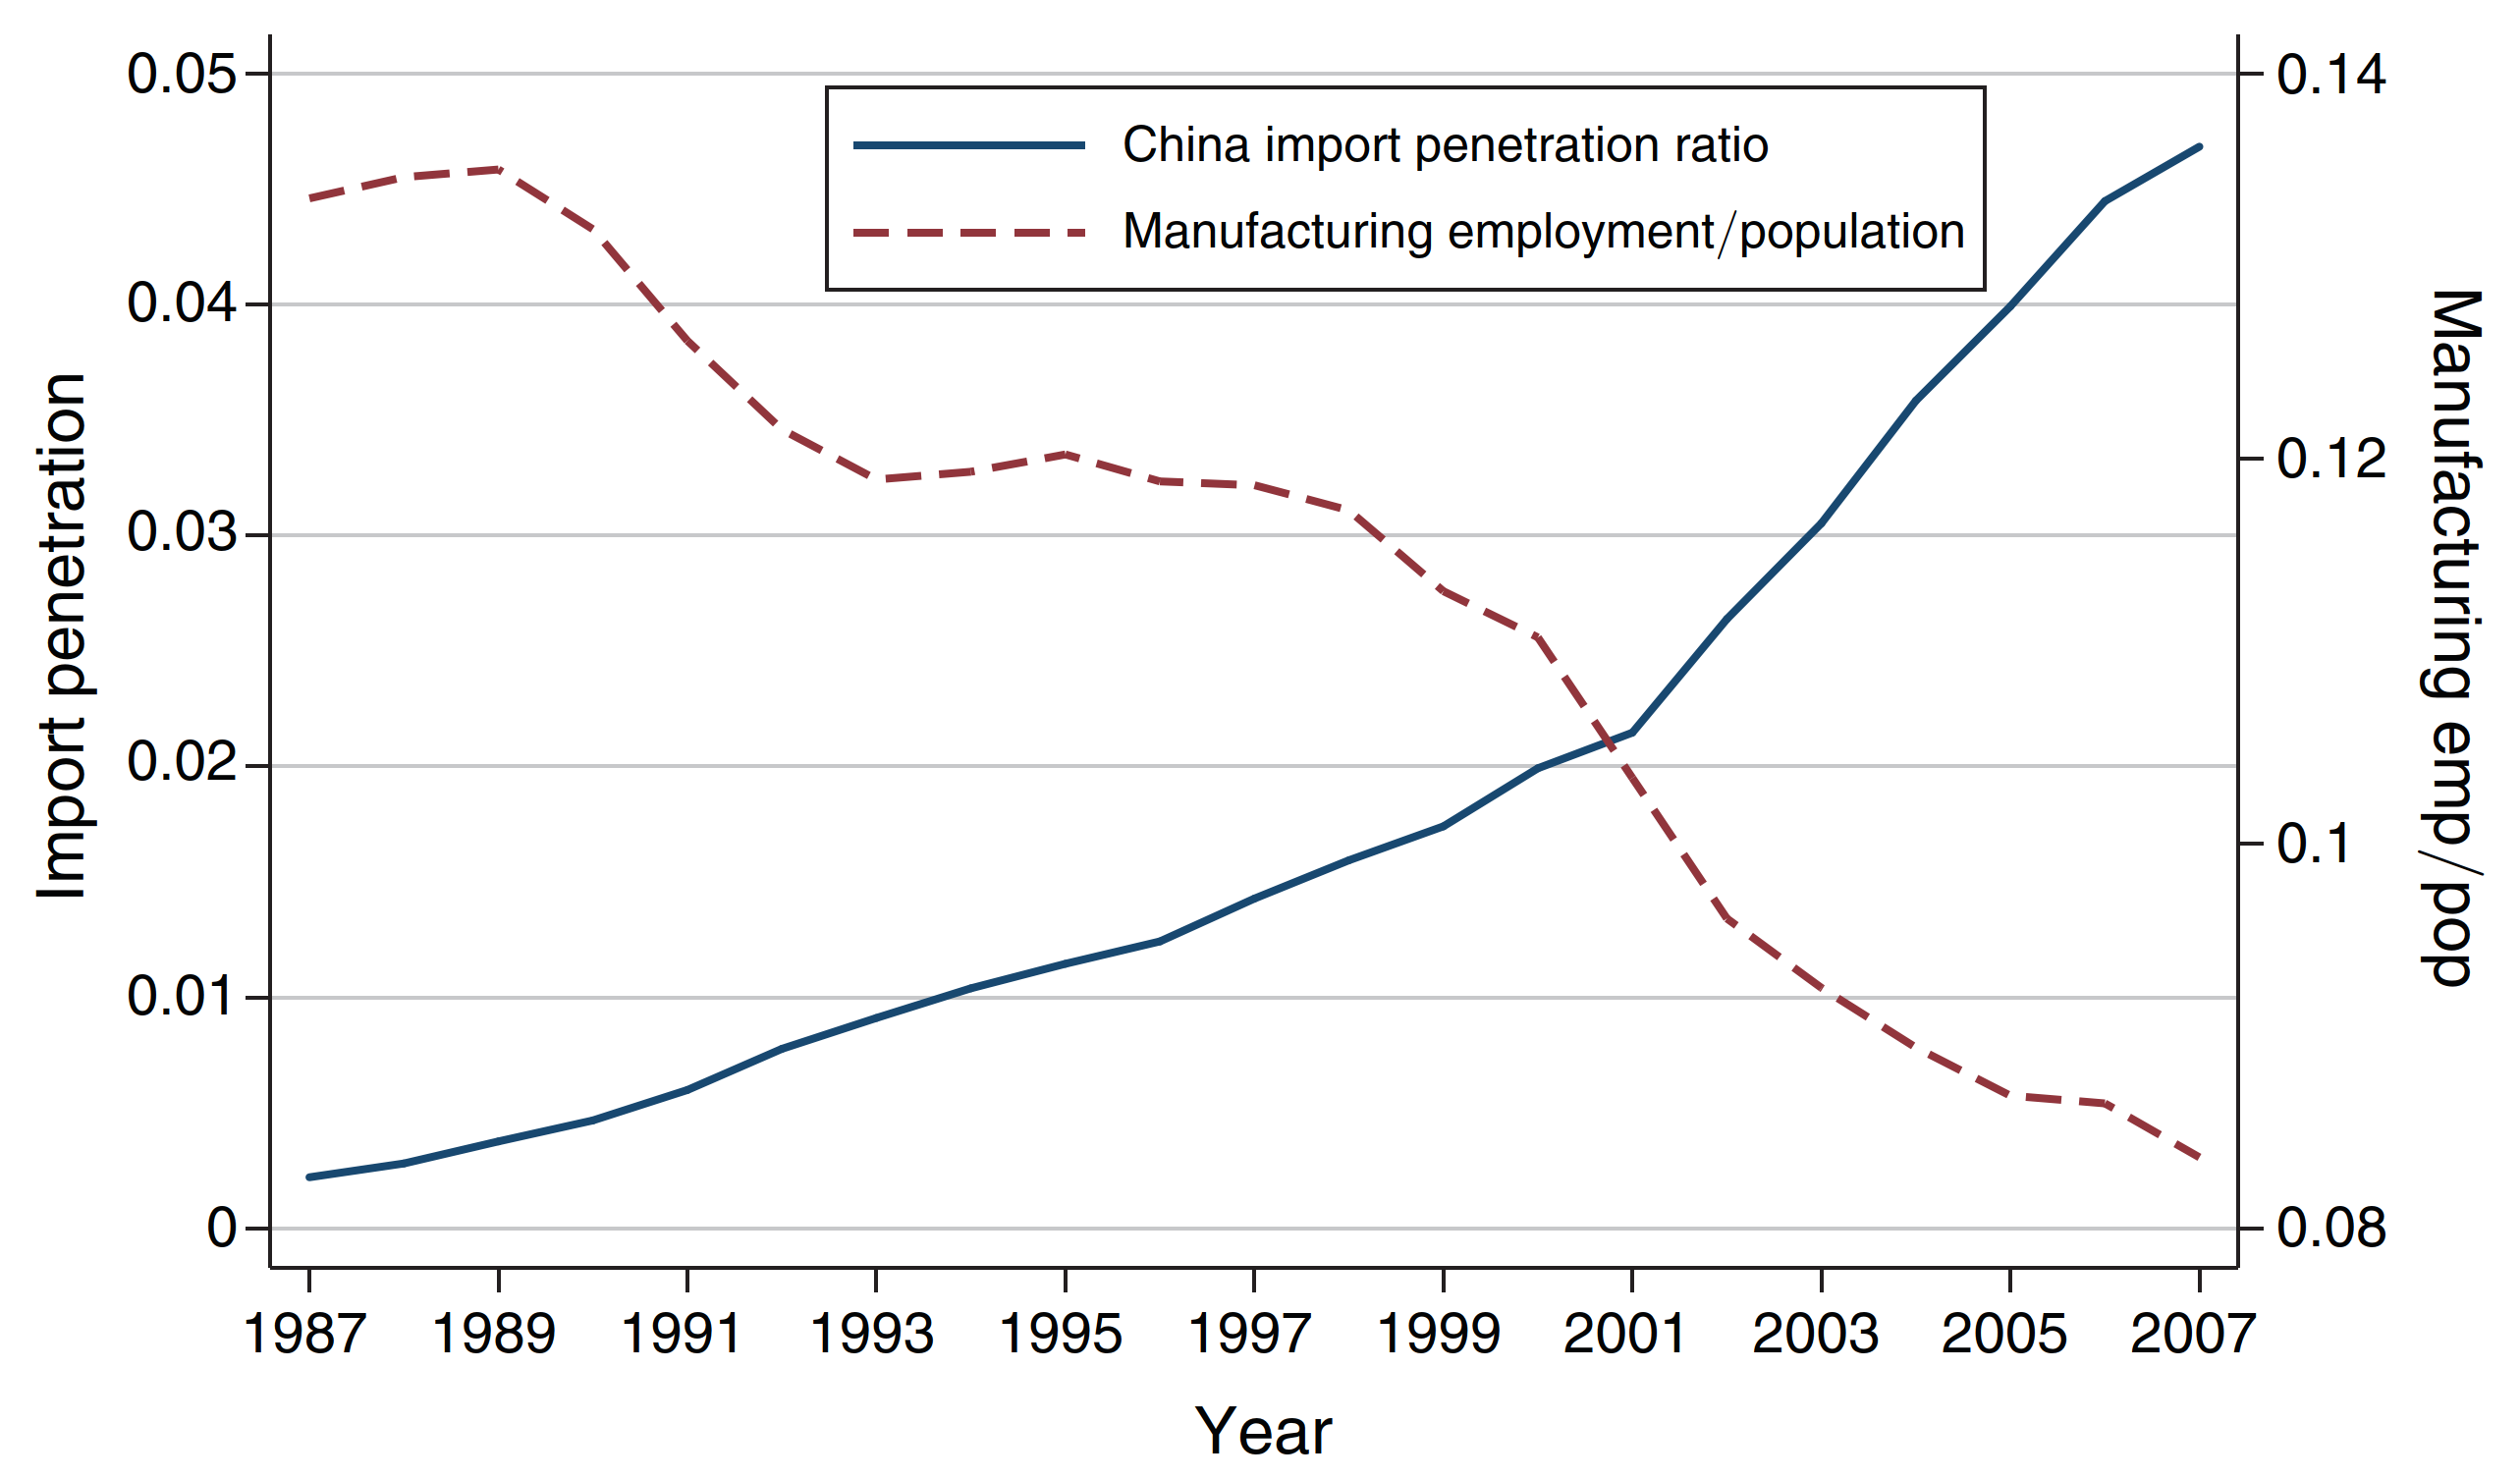
\includegraphics[width=0.85\textwidth]{figure/adh_f1.png}
		\end{figure}
	\end{center}
\end{frame}


\begin{frame}{Autor, David Dorn, and Gordon H. Hanson (2013)}{Program and Data}
	\begin{itemize}
		\item See SSIV\_build\_data.do 
				\vspace{0.2cm}
			\begin{itemize}
		\item Show how to construct shift-share IV
						\vspace{0.2cm}
			\end{itemize}
		\item See SSIV.do and SSIV.R
		\vspace{0.2cm}
		\begin{itemize}
			\item Implement IV estimation
		\end{itemize}
		\vspace{0.2cm}
		\item Use location\_level.dta
		
		
	\end{itemize}
\end{frame}




\begin{frame}{Shift-share IV design}
	\begin{itemize}
		\item Analysis is based on cross-market variations in import exposure driven by initial industry specialization.
						\vspace{0.2cm}
		\item Shift-share IV design: 
								\vspace{0.2cm}
			\begin{itemize}
		\item Changes in Chinese imports by other high-income countries, to isolate the supply-driven component of U.S. import increases.
						\vspace{0.2cm}
							\end{itemize}
		\item Focus on manufacturing industries and their local labor market conditions across U.S. regions.
	\end{itemize}
\end{frame}


\begin{frame}{Autor, David Dorn, and Gordon H. Hanson (2013)}{Step 1: Construct Treatment Variable}
%	**Independent Var: The change in import from China**
%	\small
	\begin{itemize}
		\item They use Commuting Zone (CZ) as the observation unit
							\vspace{0.2cm}
			\begin{itemize}
		\item 	CZ: multiple adjacent counties that have the commuting structure of a local labor market
									\vspace{0.2cm}
	\end{itemize}

\item The treatment variable $\Delta I P_{it}^{c u}$ measures local exposure at zone $i$ to the growth
of imports from China per worker (measured in \$1,000) during period $t$ and $t-10$


		%\item For each industry $k$ in CZ $i$, period $\tau$, period-start-year t, 

\[ \Delta I P_{it}^{c u}\,=\,\sum_{k}\overbrace{\frac{\Delta M_{kt}^{cu}}{L_{kt}}}^{shift}\overbrace{\frac{L_{i k t}}{L_{i t}}}^{share} \]
	\begin{itemize}
		
										\vspace{0.2cm}
		\item $\frac{L_{ikt}}{L_{it}}$ the industry k's employment share of zone $i$ at year t.
											\vspace{0.2cm}
											
	\end{itemize}
	\end{itemize}
\end{frame}



\begin{frame}{Autor, David Dorn, and Gordon H. Hanson (2013)}{Step 1: Construct Treatment Variable}

	\[ \Delta I P_{it}^{c u}\,=\,\sum_{k}\overbrace{\frac{\Delta M_{kt}^{cu}}{L_{kt}}}^{shift}\overbrace{\frac{L_{i k t}}{L_{i t}}}^{share} \]
	\begin{itemize}
		
		
		%\frac{\Delta M_{kt}^{cu}}{L_{kt}}
		
		\item $\frac{\Delta M_{kt}^{cu}}{L_{kt}}$ is exposure to the growth of imports from China per worker  in the industry $k$ (measured in \$1,000)
									\vspace{0.2cm}
		\begin{itemize}
\item $\Delta M^{cu}_{k\tau}$: the growth in US imports from China during period $t$ and $t-\tau$
									\vspace{0.2cm}
		\item $L_{kt}$: total employment in industry $k$ at period $t$
		\end{itemize}
		

		

	\end{itemize}
\end{frame}




\begin{frame}{Autor, David Dorn, and Gordon H. Hanson (2013)}{Step 2: Construct Shift-Share IV}
	The SSIV for this paper is: 
	\[ \Delta Z_{it}^{c o}\,=\,\sum_{k}\overbrace{\frac{\Delta M_{kt}^{co}}{L_{kt-10}}}^{shift}\overbrace{\frac{L_{i k t-10}}{L_{i t-10}}}^{share} \]

	\begin{itemize}
		
		
		

		\item \textbf{Shift part:}  $\frac{\Delta M_{kt}^{co}}{L_{kt-10}}$ 
		\vspace{0.2cm}
		\begin{itemize}
			\item $\Delta M^{co}_{kt}$: the growth in other high-income countries' imports from China during period $t$
			\vspace{0.2cm}
			\item $L_{kt-10}$: total employment in industry $k$ in period $t-10$ (lag 10 years)
		\end{itemize}
				\vspace{0.2cm}
			\item \textbf{Share part:} lag 10 years
		
%		\item $\Delta I P_{k\tau}^{c u}\;=\;\Delta M_{k\tau}^{cu}/L_{kt}$ is exposure to the growth of imports from China per worker (measured in \$1,000) in the industry $k$
%		\vspace{0.2cm}
%		
%		
%	
%		
%		
%		
%		
%		A non-US exposure variable $\Delta{IP}_{j\tau}^{co}$ that is constructed using data on industry-level growth of Chinese exports to other high-income markets
%		\item \textbf{Share part:} lag 10 years

	\end{itemize}
\end{frame}



\begin{frame}{Autor, David Dorn, and Gordon H. Hanson (2013)}{Step 2: Construct Shift-Share IV}
	
	\begin{center}
		\begin{figure}[p]
			\centering
			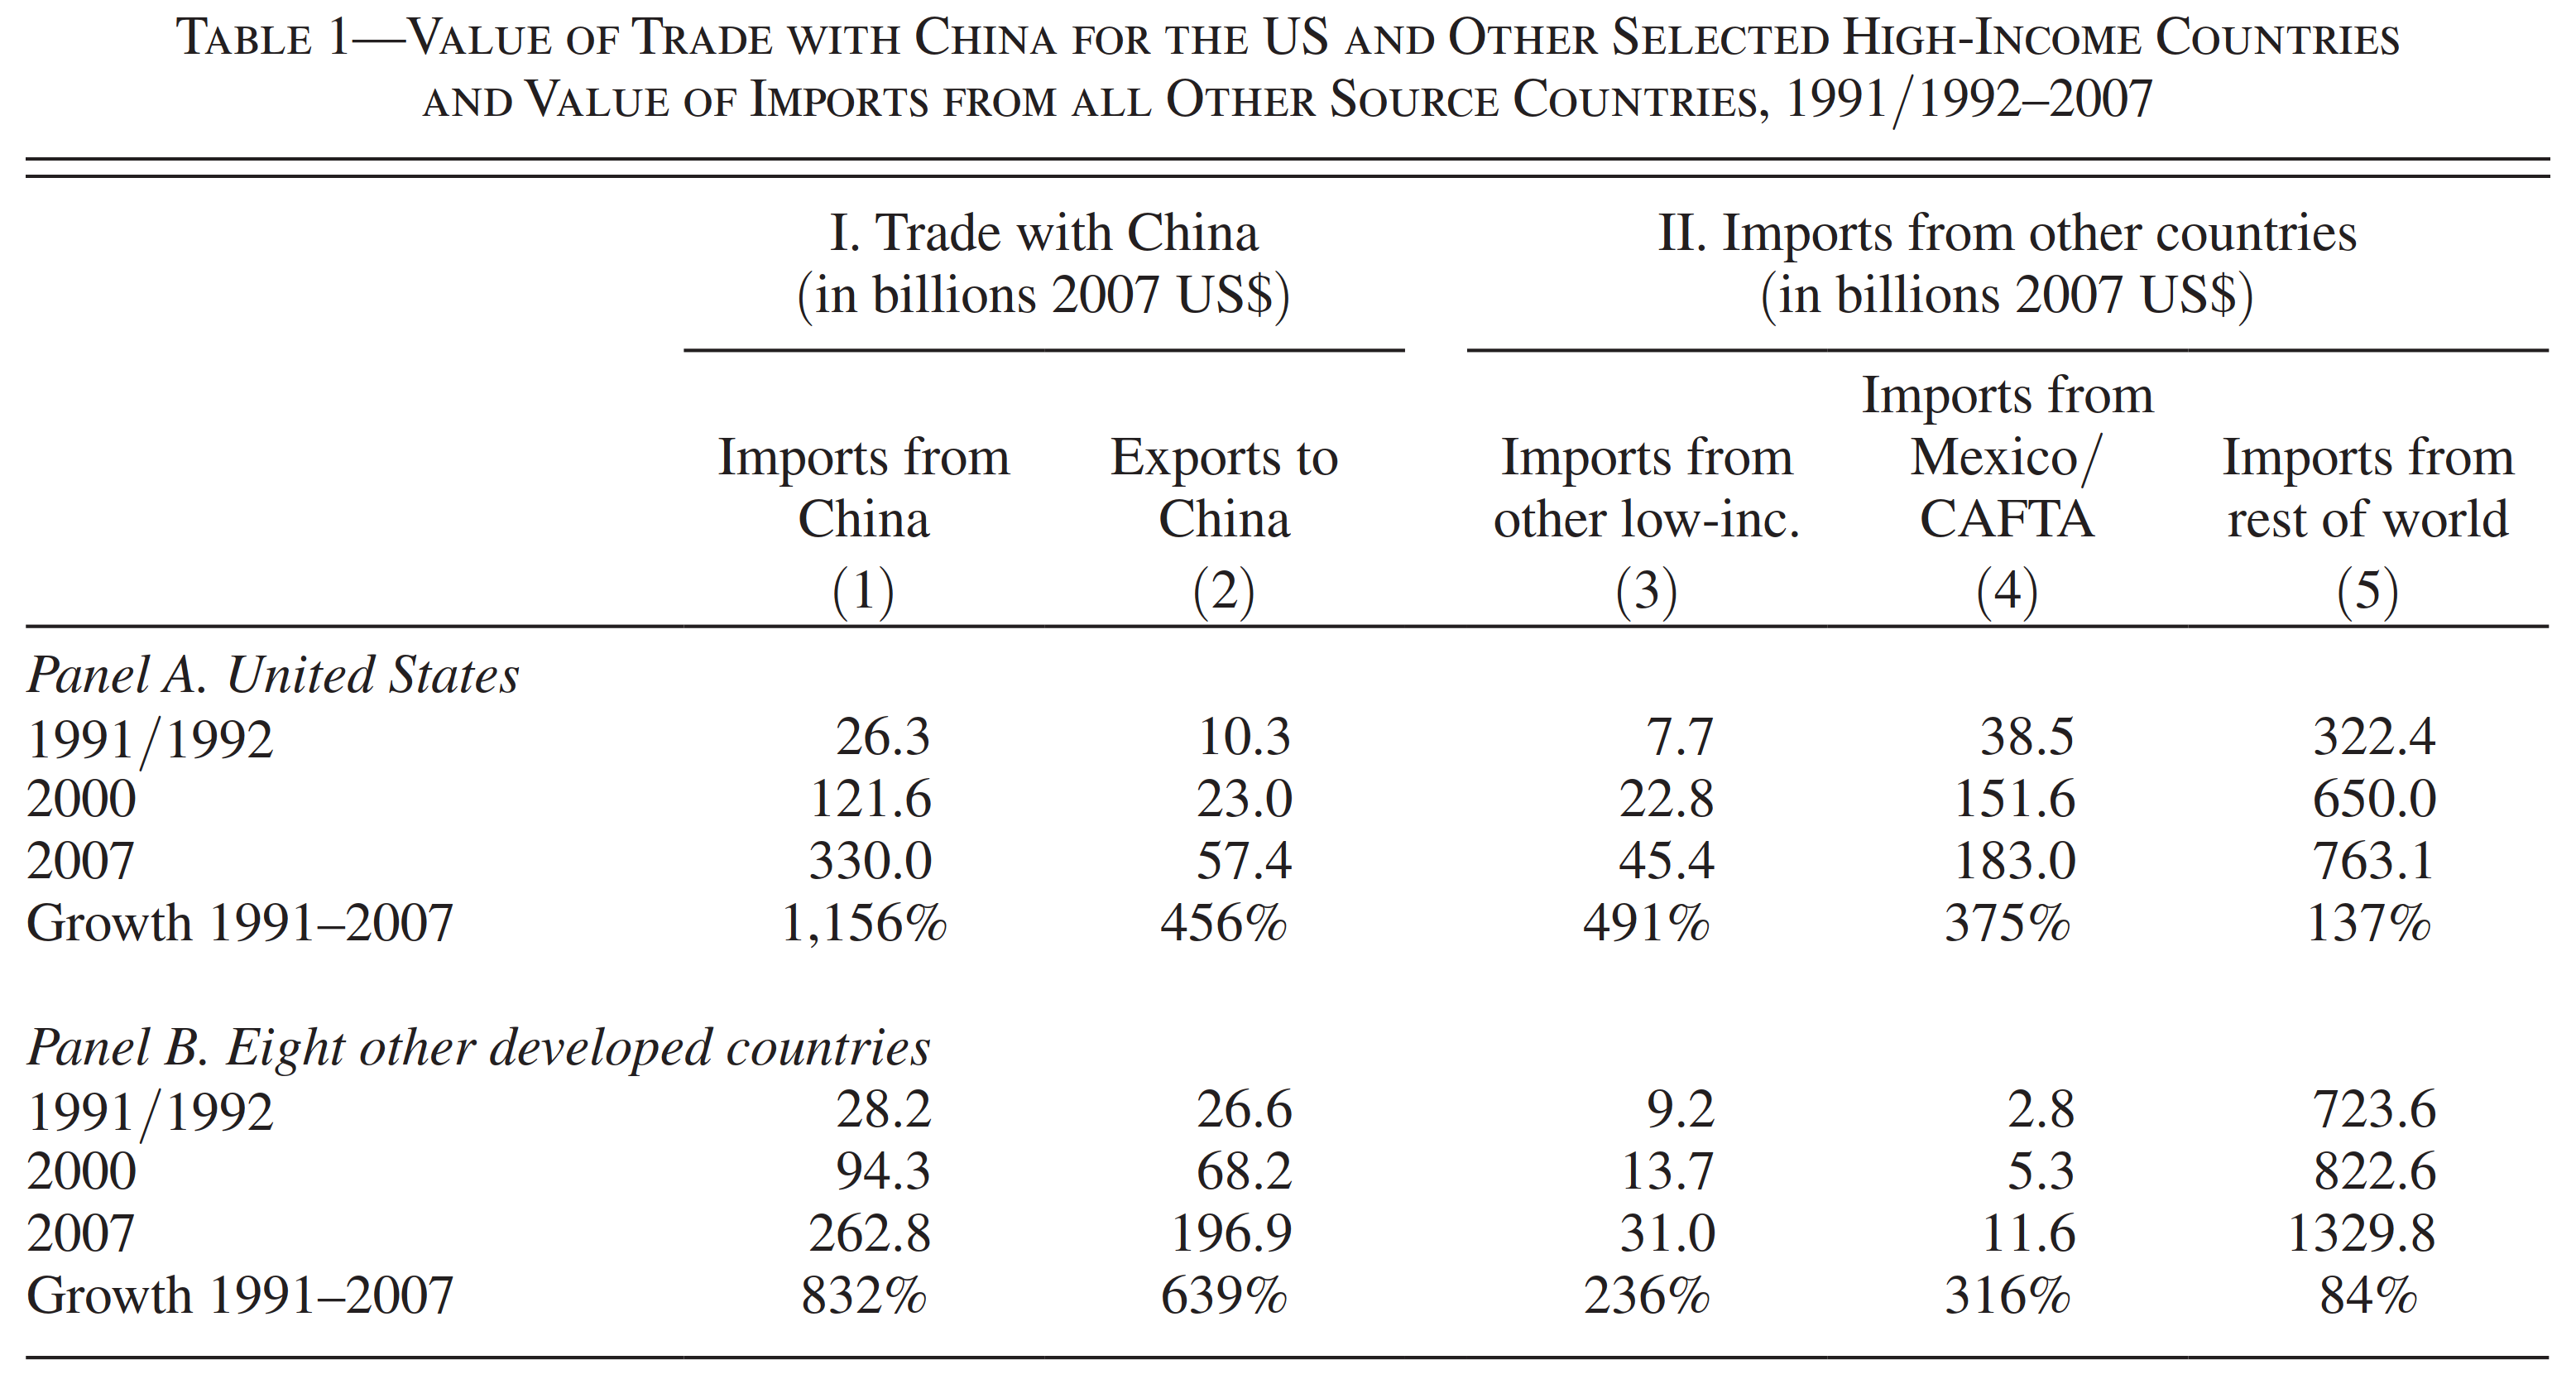
\includegraphics[width=0.85\textwidth]{figure/adh_t1.png}
		\end{figure}
	\end{center}
\end{frame}



\begin{frame}{Autor, David Dorn, and Gordon H. Hanson (2013)}{Step 3: Empirical Specification}
	\begin{itemize}
		\item \textbf{First Stage Regression:}
		\begin{equation*}
			\Delta I P_{it}^{c u} = \lambda + \alpha \Delta Z_{it}^{co} + X_{it-10} \theta +  \epsilon_{it}
		\end{equation*}
		\item \textbf{Second Stage Regression:}
		\begin{equation*}
			\Delta Y_{it} =  \kappa + \beta \Delta \hat{I P}_{i\tau}^{c u}+ X_{it-10} \gamma + u_{it}
		\end{equation*}
		
		\item Use shift-share as IV for treatment variable $\Delta I P_{i\tau}^{c u}$
		
	\[ \Delta Z_{it}^{c o}\,=\,\sum_{k}\overbrace{\frac{\Delta M_{kt}^{co}}{L_{kt-10}}}^{shift}\overbrace{\frac{L_{i k t-10}}{L_{i t-10}}}^{share} \]
		%	\item Here, \(\hat{T}\) is the predicted level of automation from the first stage.
	\end{itemize}
\end{frame}



\begin{frame}{Graphical Evidence}{}
	
	\begin{center}
		\begin{figure}[p]
			\centering
			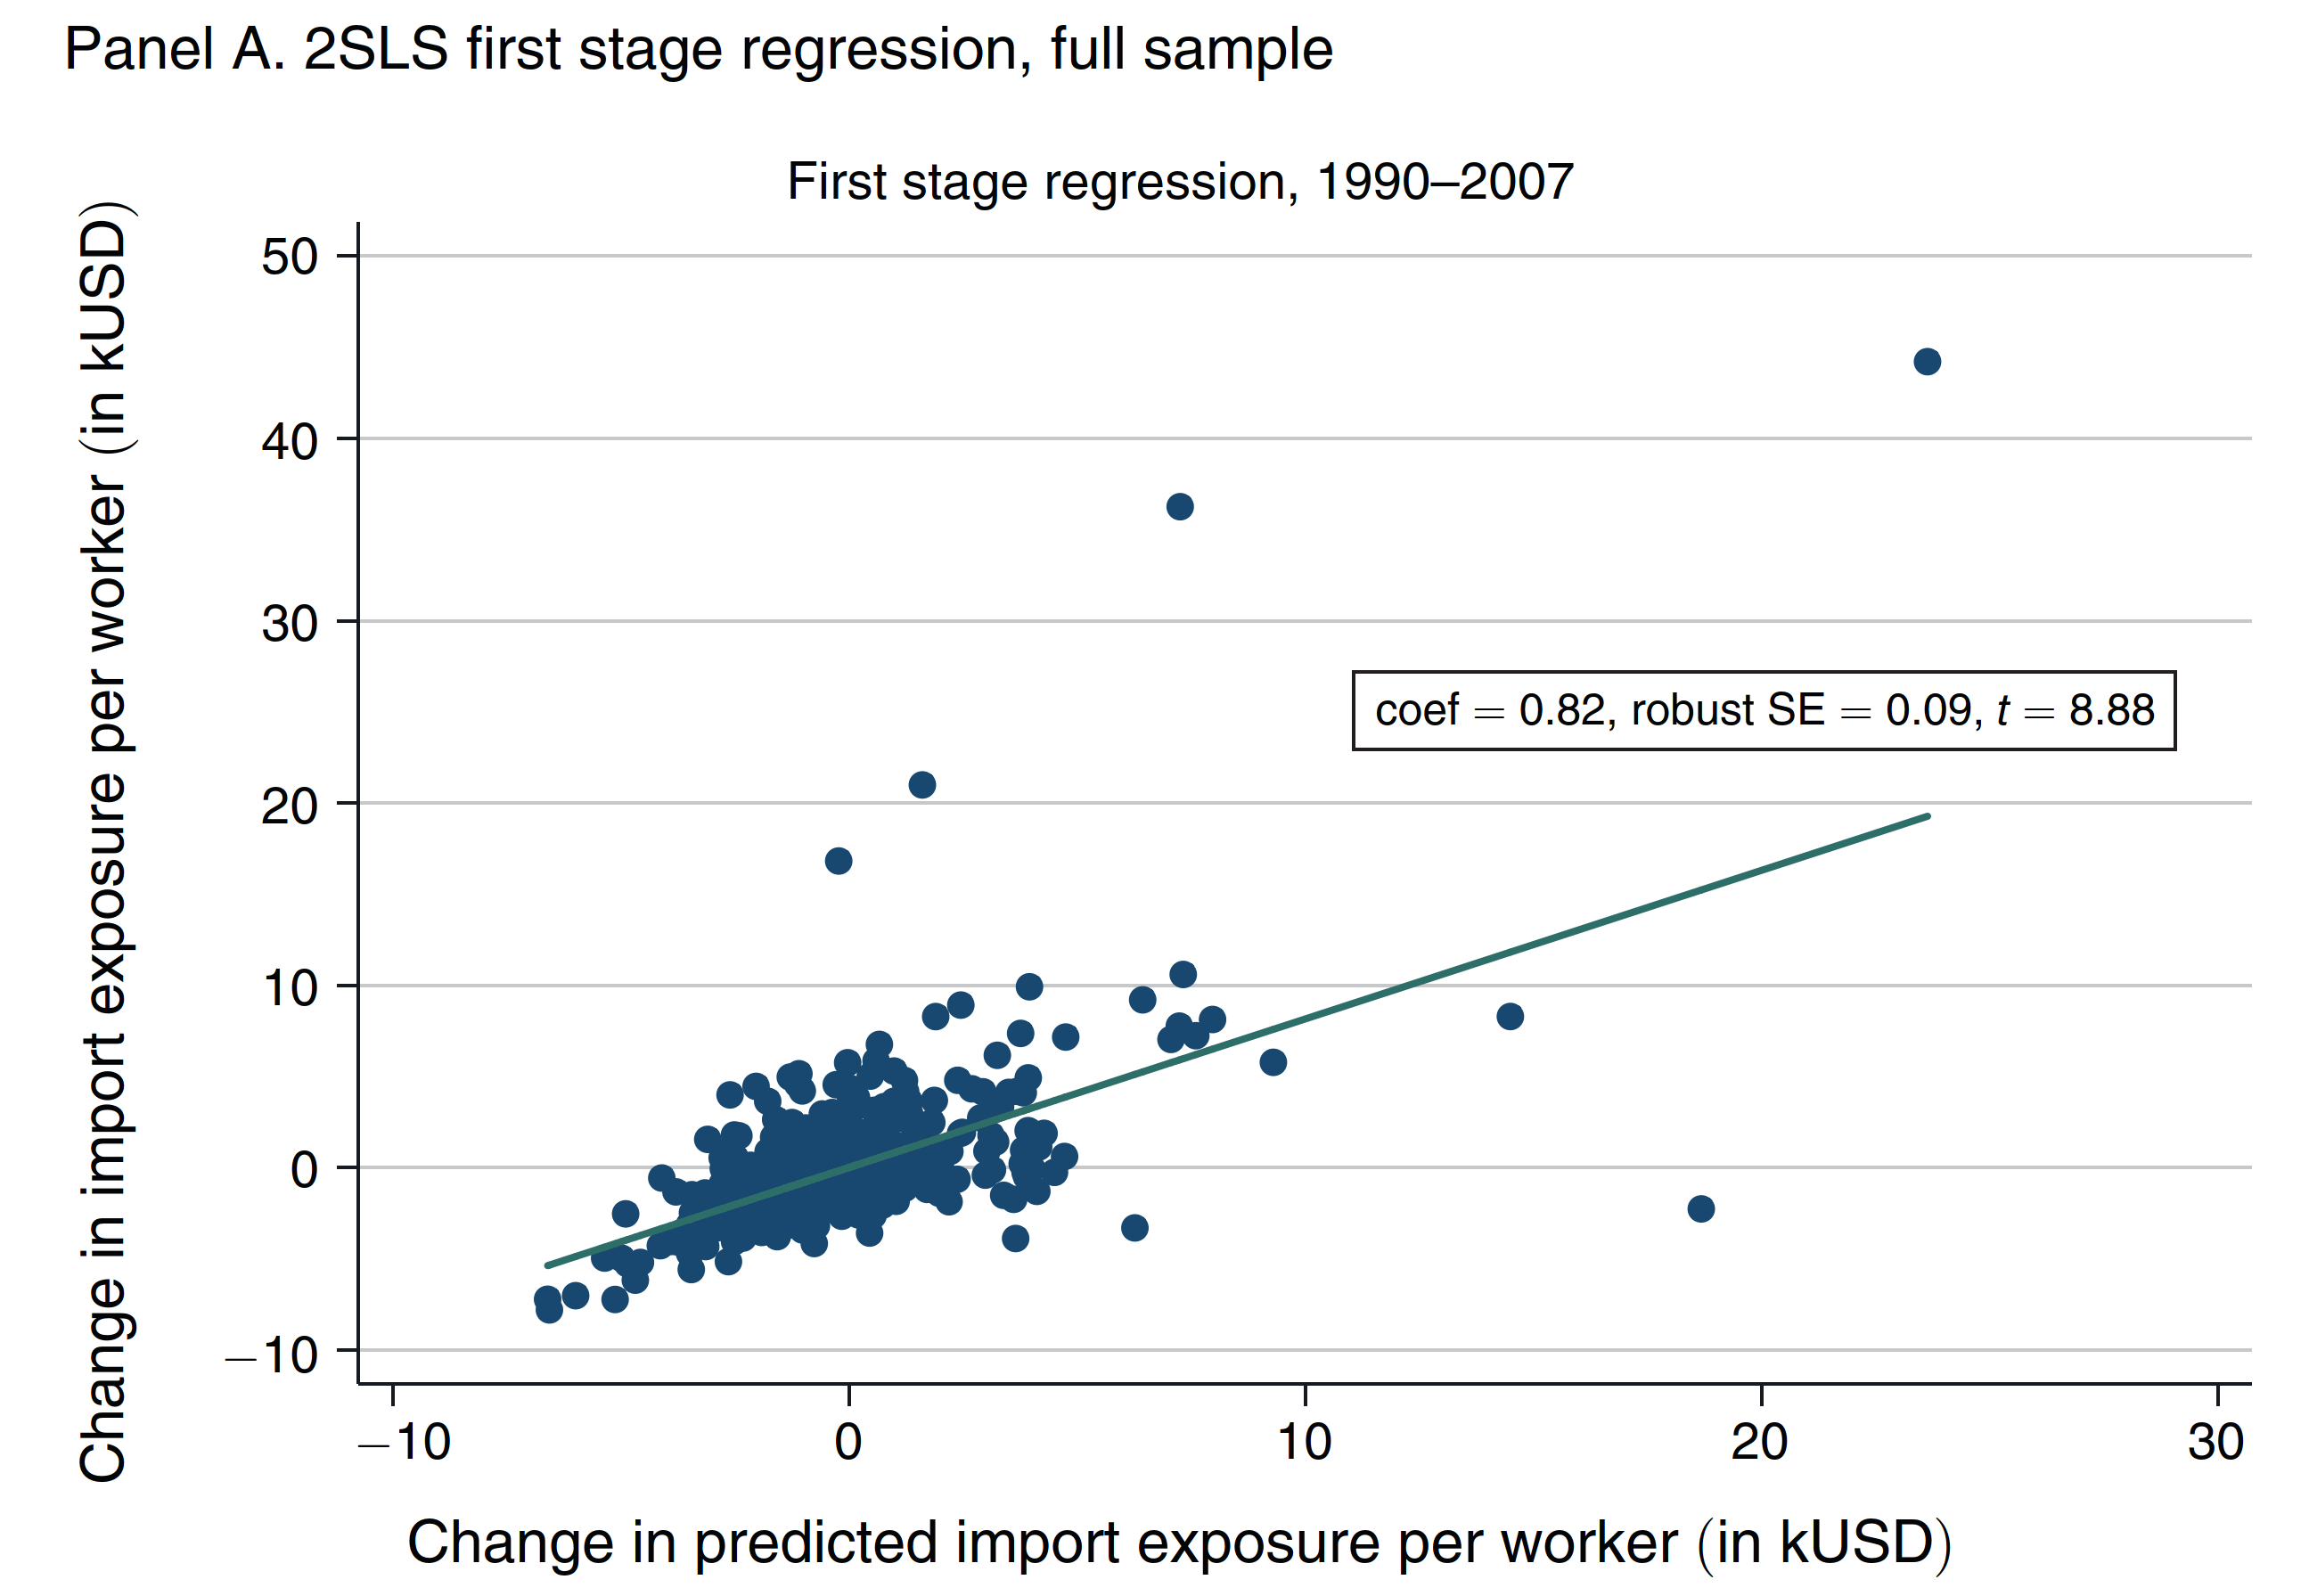
\includegraphics[width=0.85\textwidth]{figure/adh_f2a.png}
		\end{figure}
	\end{center}
\end{frame}



\begin{frame}{Graphical Evidence}{}
	
	\begin{center}
		\begin{figure}[p]
			\centering
			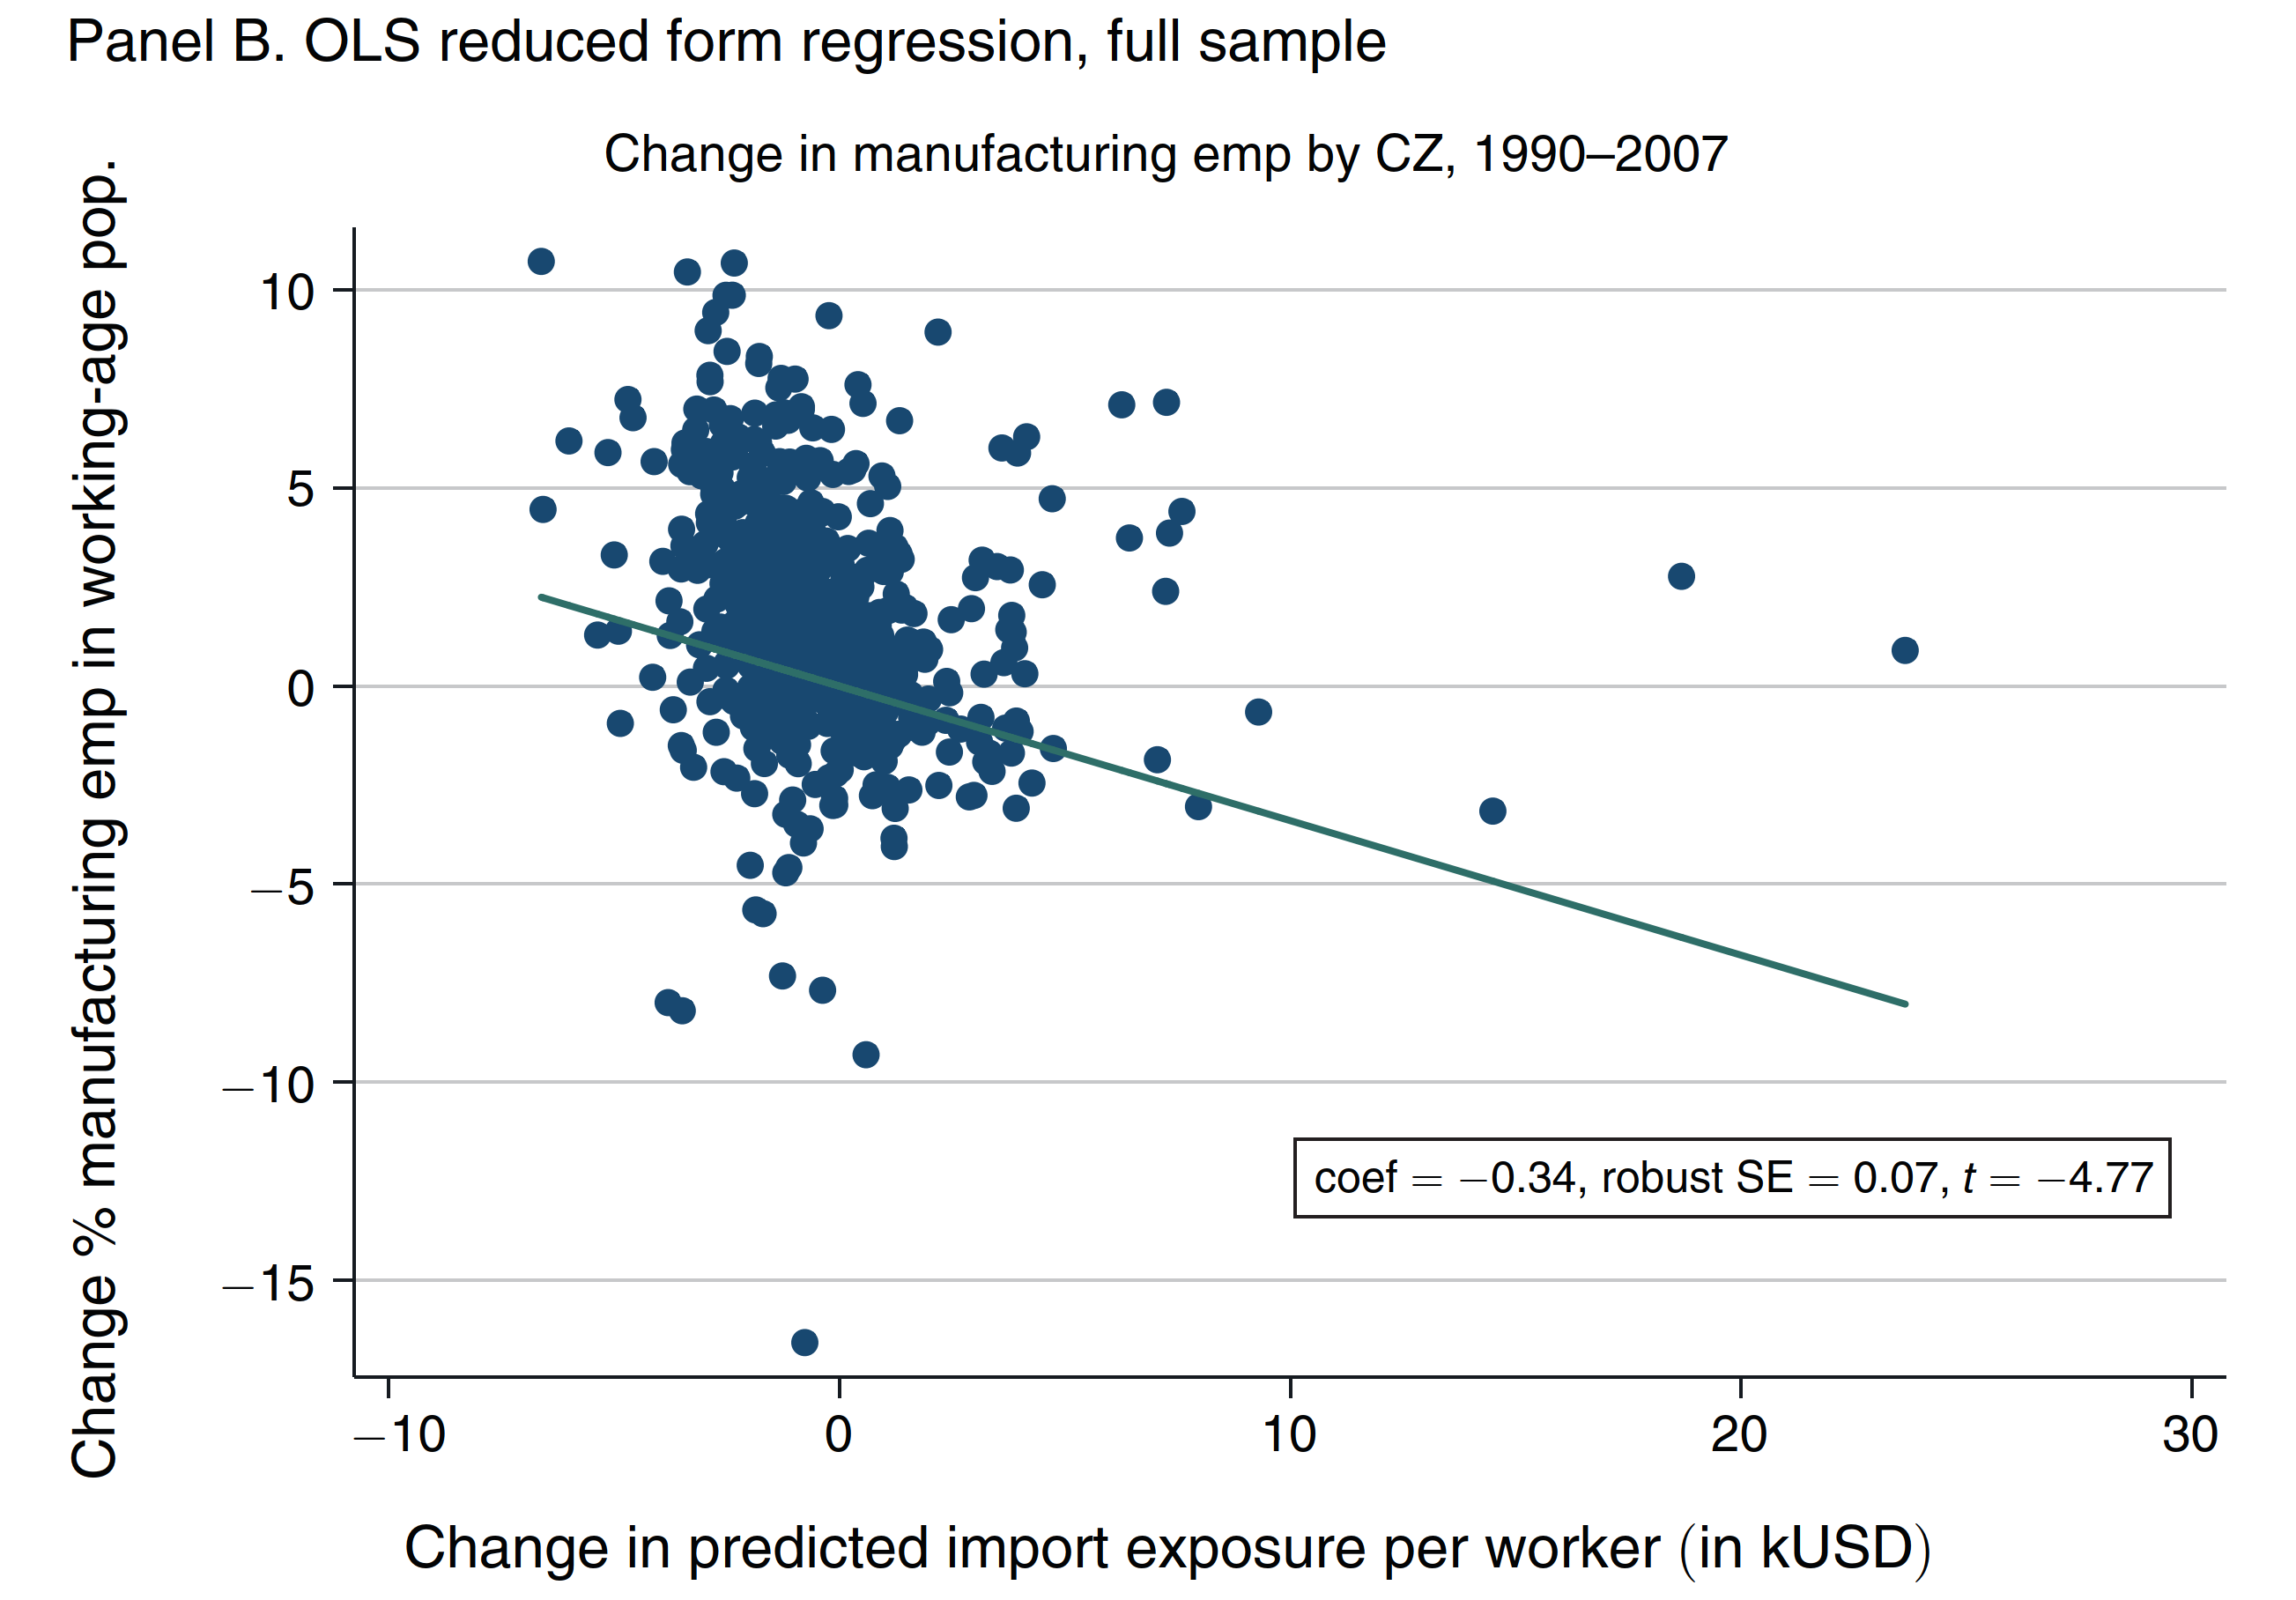
\includegraphics[width=0.85\textwidth]{figure/adh_f2b.png}
		\end{figure}
	\end{center}
\end{frame}



\begin{frame}[fragile]{STATA Command: ivregress}
	\begin{itemize}
\begin{lstlisting}
ivregress 2sls y (x=z)  [aw=wei], cluster(czone) first

ivregress 2sls y (x=z) l_sh_popedu_c l_sh_popfborn l_sh_empl_f l_sh_routine33 l_task_outsource [aw=wei], cluster(czone) first

ivreghdfe y (x=z) [aw=wei], cluster(czone)

ivreghdfe y (x=z) l_sh_popedu_c l_sh_popfborn l_sh_empl_f l_sh_routine33 l_task_outsource [aw=wei], cluster(czone)
\end{lstlisting}
		
		\vspace{0.2cm}
		\item  \textbf{aw=wei}: total employment at initial period
		\vspace{0.2cm}
		\item \textbf{y}: manufacturing employment at CZ
		\vspace{0.2cm}
		\item \textbf{x} china import exposure at CZ
		\vspace{0.2cm}
		\item \textbf{z}: shift-share IV 
	\end{itemize}
\end{frame}







%\begin{frame}[fragile]{R Command: lm}
%	\begin{itemize}
%\begin{lstlisting}
%# Basic OLS regression with clustering
%model1 <- lm(y ~ x, data = location_level, weights = wei)
%coeftest(model1, vcov = vcovCL, cluster = ~czone)
%	
%# Extended OLS regression with clustering
%model2 <- lm(y ~ x + l_sh_popedu_c + l_sh_popfborn + l_sh_empl_f + l_sh_routine33 + l_task_outsource, 
%data = location_level, weights = wei)
%coeftest(model2, vcov = vcovCL, cluster = ~czone)
%\end{lstlisting}
%		
%		\vspace{0.2cm}
%		\item  \textbf{wei}: Total employment at the initial period, used as weights in the regression
%		\vspace{0.2cm}
%		\item \textbf{y}: Manufacturing employment at the commuting zone (CZ)
%		\vspace{0.2cm}
%		\item \textbf{x}: China import exposure at the commuting zone (CZ)
%		
%	\end{itemize}
%\end{frame}



\begin{frame}[fragile]{R Command: ivreg}
	\begin{itemize}
\begin{lstlisting}
# Instrumental variables regression using ivreg
model3 <- ivreg(y ~ x | z, data = location_level, weights = wei)
summary(model3, vcov = vcovCL, cluster = ~czone)

# Instrumental variables regression with additional controls
model4 <- ivreg(y ~ x + l_sh_popedu_c + l_sh_popfborn + l_sh_empl_f + l_sh_routine33 + l_task_outsource | z, 
data = location_level, weights = wei)
summary(model4, vcov = vcovCL, cluster = ~czone)
\end{lstlisting}
		
		\vspace{0.2cm}
\item \textbf{z}: Shift-share instrument used for IV regression
\vspace{0.2cm}
		
	\end{itemize}
\end{frame}




\begin{frame}{Results}{}
	
	\begin{center}
		\begin{figure}[p]
			\centering
			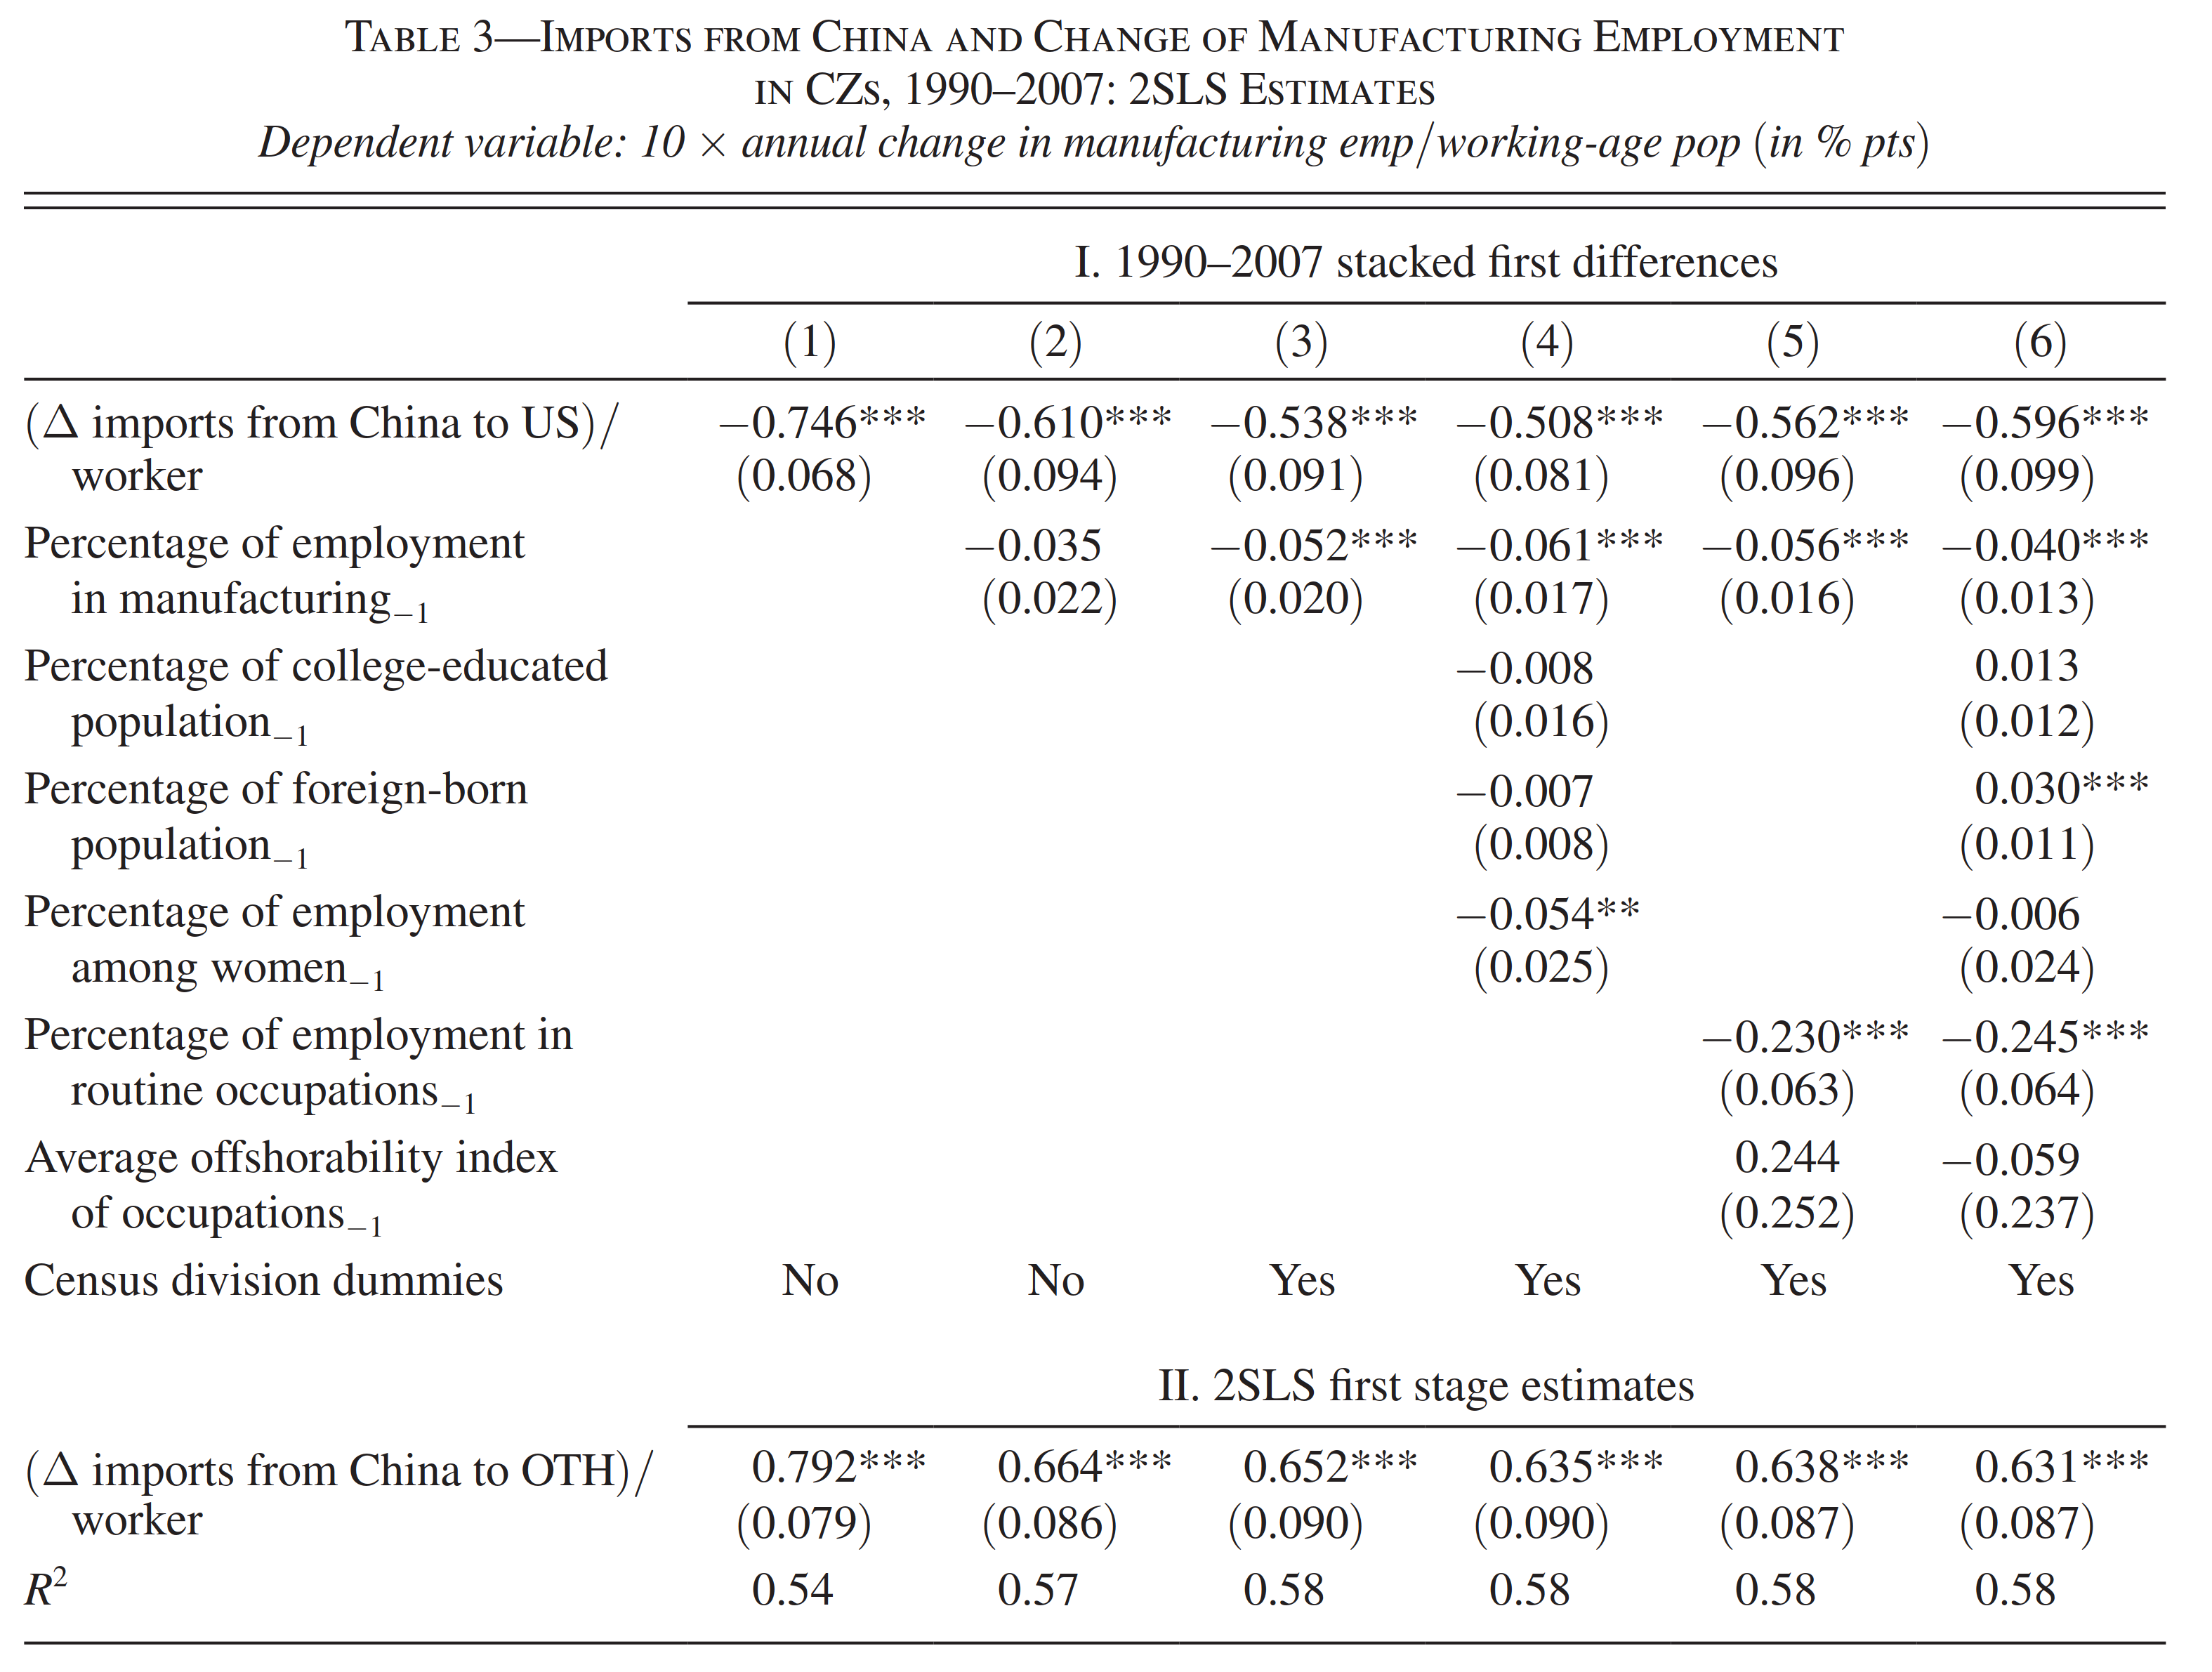
\includegraphics[width=0.85\textwidth]{figure/adh_t3.png}
		\end{figure}
	\end{center}
\end{frame}



%\begin{frame}{Results}{}
%	\begin{itemize}
%		\item Rising Chinese imports account for nearly \textbf{one-quarter to one-half} of the decline in U.S. manufacturing employment between 1990 and 2007.
%		\vspace{0.2cm}
%		\item A \$1,000 per worker increase in import exposure over a decade leads to a \textbf{0.60 percentage point} decline in the manufacturing employment share of the working-age population.
%		\vspace{0.2cm}
%		\item Areas with higher initial shares of routine-intensive jobs or manufacturing employment experience larger declines.
%		\vspace{0.2cm}
%		\item The findings highlight large \textbf{local adjustment costs} of trade: exposed regions saw \textbf{lower wages}, \textbf{reduced labor force participation}, and \textbf{greater reliance on transfer programs} (e.g., SSDI, UI).
%	\end{itemize}
%\end{frame}





\begin{frame}{Results}{}
	\begin{itemize}
		\item Rising Chinese imports account for about one-quarter of the aggregate decline in U.S. manufacturing employment.
				\vspace{0.2cm}
			\item A \$1,000 per worker increase in import exposure over a decade leads to a \textbf{0.60 percentage point} decline in the manufacturing employment share of the working-age population.
		\vspace{0.2cm}		
				
		\item Exposed regions saw higher unemployment, lower labor force participation, and reduced wages.
				\vspace{0.2cm}
		\item Government benefits (e.g., unemployment and disability) increased significantly in more exposed regions.
						\vspace{0.2cm}
			\item The findings highlight significant adjustment costs for local labor markets facing rising low-wage imports.
	\end{itemize}
\end{frame}

%\begin{frame}{Implications}
%	\begin{itemize}
%		\item The findings highlight significant adjustment costs for local labor markets facing rising low-wage imports.
%				\vspace{0.2cm}
%		\item Policy implications include the need for targeted support for adversely affected local economies.
%				\vspace{0.2cm}
%		\item Future research could explore the long-term effects of such trade shocks on regional economic resilience.
%	\end{itemize}
%\end{frame}


%\begin{frame}{Autor, David Dorn, and Gordon H. Hanson (2013)}{Step 3: Empirical Specification}
%
%	\[ \Delta Y_{c d j \tau}\:=\:\gamma\:+\:\beta_{1}\Delta I P_{j \tau}^{c u}\:+\:X_{c d j}^{\prime}\beta_{2}\:+\:e_{c d j \tau}, \]
%	\small
%	\begin{itemize}
%	\item $\Delta Y_{c d j \tau}$: change in labor market outcomes in the period $\tau$
%					\vspace{0.2cm}
%	\item $X_{c d j}^{\prime}$: including Census-division dummies, initial CZ economic and political conditions, and demographic characteristics
%					\vspace{0.2cm}
%	\item **start-of-period manufacturing share within CZs** (see next page)
%\end{itemize}
%\end{frame}
%
%
%\begin{frame}{Autor, David Dorn, and Gordon H. Hanson (2013)}{Step 3: Empirical Specification}
%	In Autor et al. (2022): The variation of indep var arises from two sources:
%	\begin{itemize}
%		\item differential concentration of employment in manufacturing versus nonmanufacturing activities
%		\item specialization in import-intensive industries within local manufacturing.
%	\end{itemize}
%	In their main specifications, they control for the start-of-period manufacturing share within CZs so as to \textit{focus on variation in exposure to trade arising from differences in industry mix within local manufacturing.} (Me: Weird...)
%\end{frame}


	\begin{frame}{Suggestive Readings}
	\tiny
	\begin{itemize}
		\item Mckenzier David. 2018. \textit{``Rethinking identification under the Bartik Shift-Share Instrument."} \href{https://blogs.worldbank.org/impactevaluations/rethinking-identification-under-bartik-shift-share-instrument}{World Bank blog}
		\item Byrne, Ieran, Florence Kondylis and John Loeser. 2021. \textit{``Just a little Bartik exposure."} \href{https://blogs.worldbank.org/impactevaluations/just-little-bartik-exposure}{World Bank Blog}
		\item Autor, D., Dorn, D., Hanson, G., & Majlesi, K. 2020. \textit{``Importing political polarization? The electoral consequences of rising trade exposure."} American Economic Review, 110(10), 3139-3183.
		\item Ferri, Benjamin. 2022. \textit{``Novel Shift-Share Instruments and Their Applications",} No 1053, Boston College Working Papers in Economics, Boston College Department of Economics
		\item Adão, Rodrigo, Michal Kolesár, and Eduardo Morales. 2019. \textit{``Shift-Share Designs: Theory and Inference."} Quarterly Journal of Economics, 134(4): 1949–2010.
		\item Bartik, Timothy. 1991. \textit{``Who Benefits from State and Local Economic Development Policies?"} Kalamazoo, MI: W.E. Upjohn Institute for Employment Research.
		\item Blanchard, Olivier, and Lawrence Katz. 1992. \textit{``Regional Evolutions."} Brookings Papers on Economic Activity, 23(1): 1–76.
		\item Borusyak, Kirill, Peter Hull, and Xavier Jaravel. 2022. \textit{``Quasi-Experimental Shift-Share Research Designs."} The Review of Economic Studies, 89(1): 181–213.
		\item Boustan, Leah, Fernando V Ferreira, Hernan Winkler, and Eric M Zolt. 2013. \textit{``The Effect of Rising Income Inequality on
			
			Taxation and Public Expenditures: Evidence from U.S. Municipalities and School Districts, 1970-2000."} The Review of Economics and Statistics, 95(1291).
		\item Card, David. 2001. \textit{``Immigrant Inflows, Native Outflows, and the Local Labor Market Impacts of Higher Immigration."} Journal of Labor Economics, 19(1): 22–64.
		\item Goldsmith-Pinkham, Paul, Isaac Sorkin, and Henry Swift. 2020. \textit{``Bartik Instruments: What, When, Why, and How."} American Economic Review, 110(8): 2586–2624.
		\item Nunn, Nathan, and Nancy Qian. 2014. \textit{``US Food Aid and Civil Conflict."} American Economic Review, 104(6): 1630–1666.
	\end{itemize}
\end{frame}


	
%	\begin{frame}{SSIV Estimation Formula}
%		\begin{itemize}
%			\item The SSIV estimator \(\beta_1\) can be represented as:
%			\[ \beta_1 = \frac{Cov(Y, Z)}{Cov(T, Z)} \]
%			\item This formula shows the treatment effect of automation on employment, instrumented by the predicted automation.
%		\end{itemize}
%	\end{frame}
%	
%	\begin{frame}{Assumptions for Validity}
%		\begin{itemize}
%			\item \textbf{Relevance:} The instrument must be strongly correlated with the actual level of automation.
%			\item \textbf{Exogeneity:} The instrument affects employment only through its effect on automation, not directly or through omitted variables.
%		\end{itemize}
%	\end{frame}
%	
%	\begin{frame}{Conclusion}
%		\begin{itemize}
%			\item SSIV provides a robust method to identify causal effects in settings where traditional methods might fail due to endogeneity.
%			\item It is particularly useful in economic geography and labor economics where regional and industry-specific variations are significant.
%		\end{itemize}
%	\end{frame}
%	

	
	
	\end{document}	